\documentclass[xcolor=dvipsnames]{beamer} % dvipsnames gives more built-in colors
\mode<presentation>

\usetheme{Boadilla}

\definecolor{GWdarkblue}{HTML}{033C5A}

\usecolortheme[named=GWdarkblue]{structure}

% Sets the font
\usepackage[defaultfam,tabular,lining]{montserrat}
\setbeamerfont{title}{shape=\scshape}
\setbeamerfont{frametitle}{shape=\scshape}
%Remove "Figure" from captions
\setbeamertemplate{caption}{\raggedright\insertcaption\par}

\usepackage{graphicx}
\usepackage{tabularx}
\usepackage{hyperref}

\title[Data Ethics]{Data Ethics}
\author[SMPA 2152]{Data Analysis for Journalism and Political Communication (Spring 2024)}
\date{Prof. Bell}

\begin{document}

%%%%%%%%%%%%%%%%%%%%%%%%%%%%%%%%%%%%%%%%%%%%%%%%%%%%%%%%%%%%%%%%%%
\frame{
\titlepage
}


%%%%%%%%%%%%%%%%%%%%%%%%%%%%%%%%%%%%%%%%%%%%%%%%%%%%%%%%%%%%%%%%%%
\frame{\frametitle{Bouie, ``Quantifying the Pain of Slavery''}

\centering
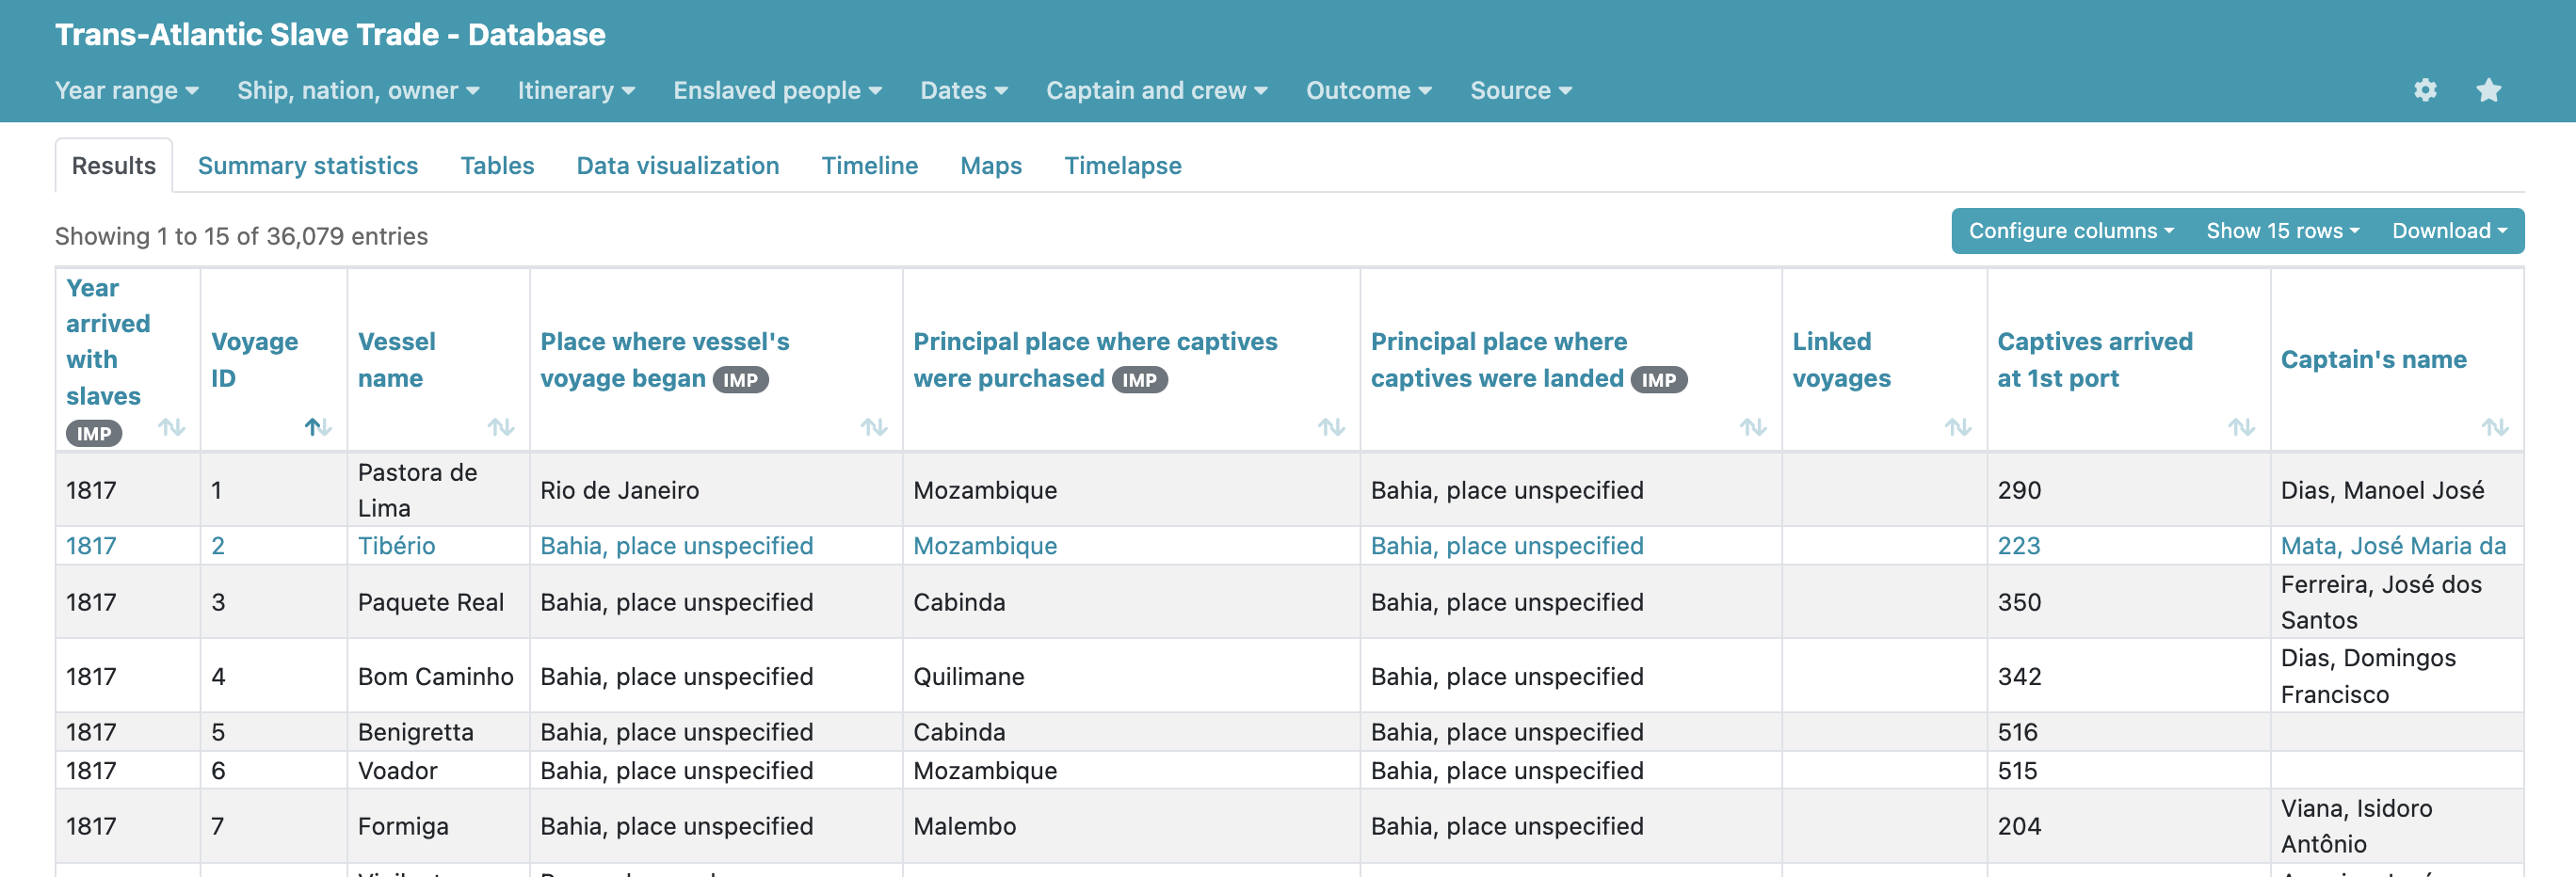
\includegraphics[height=.4\textheight]{slave_voyages.png}\\
~\\

Go to \href{https://www.slavevoyages.org/}{SlaveVoyages.org} and spend a few minutes exploring the data. Think about the implications of collecting and sharing this data. What are some of the benefits of sharing this data? What are some of the risks? Do the benefits outweigh the harms?
}

%%%%%%%%%%%%%%%%%%%%%%%%%%%%%%%%%%%%%%%%%%%%%%%%%%%%%%%%%%%%%%%%%%
\frame{\frametitle{Tuskegee Syphilis Study}
\centering
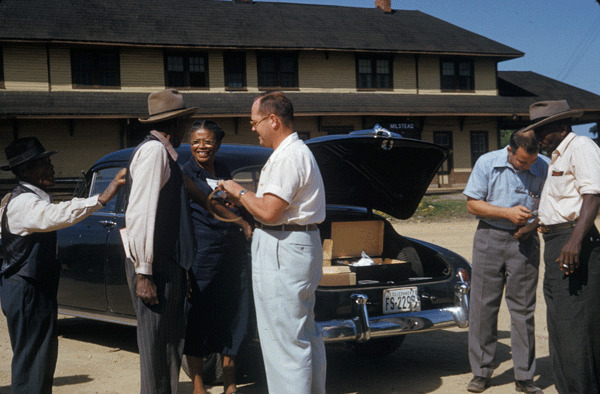
\includegraphics[width=.8\textwidth]{tuskegee}
}

%%%%%%%%%%%%%%%%%%%%%%%%%%%%%%%%%%%%%%%%%%%%%%%%%%%%%%%%%%%%%%%%%%
\frame{\frametitle{The Belmont Report (1978)}
\only<1-2>{
    \begin{itemize}[<+->]
        \item Summarizes ethical principles and guidelines for conducting research with human subjects
        \item Codified into law as the ``Common Rule'', which covers all federally-funded research
    \end{itemize}
}
\only<3->{
\begin{block}{Respect for Persons}
    Individuals should be treated as autonomous agents, and persons with diminished autonomy are entitled to protection.
\end{block}
}
\vfill
\only<4->{
\begin{block}{Beneficence}
     (1) Do not harm and (2) maximize possible benefits and minimize possible harms.
\end{block}
}
\vfill
\only<5>{
\begin{block}{Justice}
     Groups who bear the burden of research should also be the beneficiaries of that research.
\end{block}
}
}

%%%%%%%%%%%%%%%%%%%%%%%%%%%%%%%%%%%%%%%%%%%%%%%%%%%%%%%%%%%%%%%%%%
\frame{\frametitle{Other Considerations}
\begin{itemize}[<+->]
    \item Informed Consent
    \begin{itemize}
        \item<.-> Subjects must affirmatively agree to participate in research
        \item Participants must have all information necessary to make an informed decision
        \item What about studies that require deception? Studies that compensate participants?
    \end{itemize}
    \item Weighing benefits and risks of research
    \begin{itemize}
        \item<.-> Is there a way to gain the information sought in the study that minimizes risk?
        \item If risks cannot be reduced, how great is the potential benefit to society and to the subject?
        \item Examples: Stanford Prison Experiment, Milgram Experiment
        \item[] vs. randomized drug trials, ``challenge'' trials in medicine
    \end{itemize}
    \item Selection of subjects
    \begin{itemize}
        \item<.-> Do not select favored subjects for highly beneficial research and unfavored subjects for risky research
    \end{itemize}
\end{itemize}

}

%%%%%%%%%%%%%%%%%%%%%%%%%%%%%%%%%%%%%%%%%%%%%%%%%%%%%%%%%%%%%%%%%%
\frame{\frametitle{Example: Project Nightingale}

In 2019, the \textit{Wall Street Journal} reported that the nation's second-largest health care provider, Ascension, provided Google with access to tens of millions of health records to develop AI tools that ``make health records more useful, more accessible, and more searchable.''

\begin{itemize}[<+(1)->]
    \item There was no informed consent from patients
    \item There is potential harm from the release of health records
    \item Google claims that the data was sufficiently protected and staff properly trained
    \item Improving health care is a general societal good
    \item Because there is no ``opt-in,'' the data is not biased in favor of certain demographic groups
    \item There are financial benefits that accrue to the companies, not the research subjects
\end{itemize}
}

%%%%%%%%%%%%%%%%%%%%%%%%%%%%%%%%%%%%%%%%%%%%%%%%%%%%%%%%%%%%%%%%%%
\frame{\frametitle{Case Studies}
\large
\only<1,3>{
\begin{enumerate}
    \item Home DNA Testing
    \item Crisis Text Line
    \item Diversity in Faces (DiF) dataset
\end{enumerate}
}

\only<2>{
\begin{enumerate}
    \item What are the relevant ethical principles and practices in this case?
    \item In what ways/why are there concerns about a violation of ethical principles in this case?
    \item What are some ways that data could have been used more ethically in this case?
\end{enumerate}
}
}

%%%%%%%%%%%%%%%%%%%%%%%%%%%%%%%%%%%%%%%%%%%%%%%%%%%%%%%%%%%%%%%%%%
\frame{\frametitle{De-identification}
\begin{itemize}[<+->]
    \item Researchers often promise \textbf{\textit{anonymity}} or \textbf{\textit{confidentiality}} to participants in order to reduce the risks of participating in research
    \item There are two types of identifiers that must be removed before sharing this data:
    \begin{enumerate}
        \item \textbf{Direct identifiers}: information that would be sufficient on its own to disclose an identity, such as names, addresses, and phone numbers.
        \item \textbf{Indirect identifiers}: information that \textit{in combination} would be sufficient to disclose an identity
    \end{enumerate}
    \item Examples: credit card transactions, Netflix movie ratings, tennis match-fixing
    \item De-identification is the process of removing direct and indirect identifiers
\end{itemize}
}

%%%%%%%%%%%%%%%%%%%%%%%%%%%%%%%%%%%%%%%%%%%%%%%%%%%%%%%%%%%%%%%%%%
\frame{\frametitle{De-identification}

\begin{enumerate}[<+->]
    \item Remove direct identifiers
    \item Aggregate or reduce the precision of a variable
    \begin{itemize}
        \item<.-> Generalize the meaning of categories
        \item Collapse categories
        \item Restrict the upper or lower ranges
    \end{itemize}
    \item Anonymize keys that link to other datasets
    \item Maintain a master log of all replacements, aggregations, or removals and keep it in a secure location separate from the de-identified data files
\end{enumerate}

\only<1>{
\centering
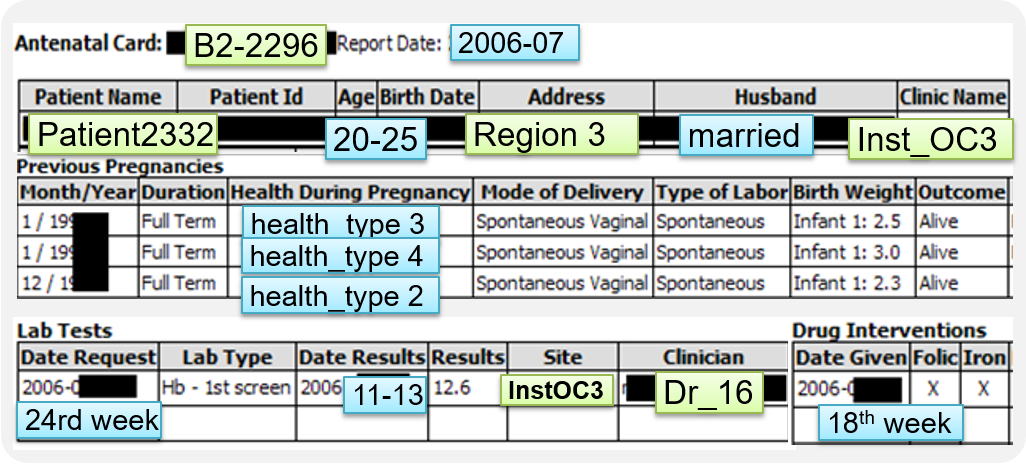
\includegraphics[height=.33\textheight]{remove_direct_identifiers.png}
}
\only<2>{
\centering
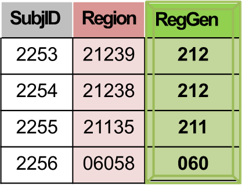
\includegraphics[height=.33\textheight]{generalize_categories.png}
}
\only<3>{
\centering
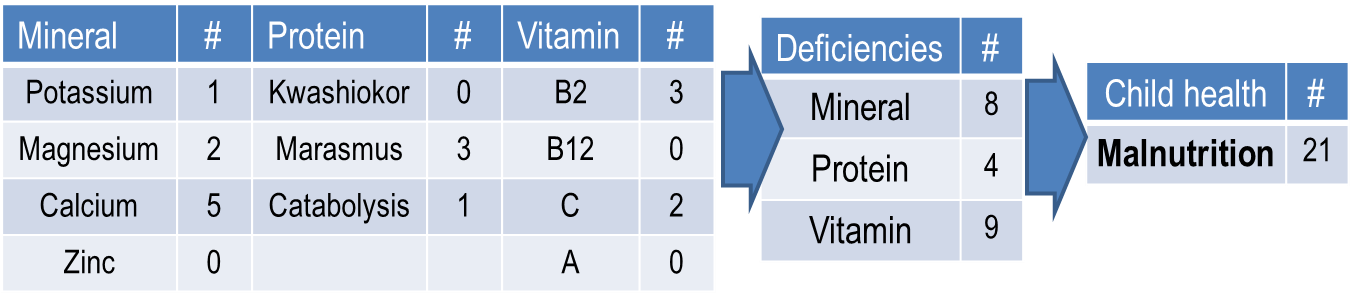
\includegraphics[height=.25\textheight]{collapse_categories.png}
}
\only<4>{
\centering
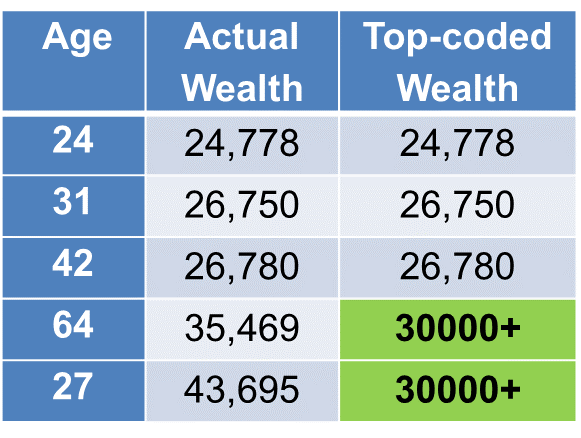
\includegraphics[height=.33\textheight]{top-code.png}
}
\only<5->{
~\\
\centering
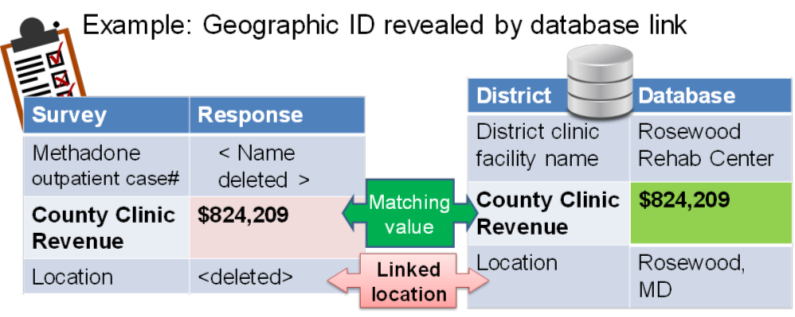
\includegraphics[height=.33\textheight]{remove_relational_links.png}
}
}

%%%%%%%%%%%%%%%%%%%%%%%%%%%%%%%%%%%%%%%%%%%%%%%%%%%%%%%%%%%%%%%%%%
\frame{\frametitle{De-identification Exercise}

}

\end{document}
